\documentclass[11pt]{article}

\usepackage[a4paper,margin=1in]{geometry}
\usepackage[T1]{fontenc}
\usepackage[utf8]{inputenc}
\usepackage{lmodern}
\usepackage{amsmath}
\usepackage{booktabs}
\usepackage{tabularx}
\usepackage{graphicx}
\usepackage{caption}
\usepackage{setspace}
\usepackage[authoryear,round]{natbib}
\usepackage[hidelinks]{hyperref}

\newcommand{\rupee}{INR~}
\onehalfspacing

\title{Does a Popular Trading Signal Beat Buy-and-Hold?\\
\large Survivorship-Free Evidence on the Triple Supertrend from the Nifty 50, 2010--2026}

% TODO: replace with your name, affiliation and e-mail before submitting.
\author{Author Name\thanks{Affiliation. E-mail: author@example.com.
This is a working paper; comments are welcome. This paper is research, not investment advice.}}

\date{October 2026}

\begin{document}
\maketitle

\begin{abstract}
\noindent
The Triple Supertrend, a trend-following rule that trades only when three Average True Range bands agree, is
widely used by Indian retail traders. We test it on an equal-weighted portfolio of the stocks that were
members of the Nifty~50 on each day from January 2010 to October 2026, using National Stock Exchange (NSE)
end-of-day files adjusted for splits, bonuses, rights issues, demergers and dividends with NSE's own
corporate-action records. The panel covers 99.3\% of index member-days, including companies later delisted.
Parameters are chosen on 2010--2018 and tested unchanged on 2019--2026. Out of sample, the strategy returns
8.0\% a year against 15.1\% for buy-and-hold, with volatility of 8.5\% against 17.4\% and a maximum drawdown of
$-12.1\%$ against $-38.6\%$. The Sharpe ratios (0.96 and 0.90) are statistically indistinguishable. Back-filling
today's constituents overstates buy-and-hold returns by 7--10 percentage points a year. A cross-sectional
momentum rule that holds the ten strongest members also beats buy-and-hold in sample but trails it out of sample
(9.3\% a year), and buying index options on the Supertrend signals loses money in simulation. The rule behaves as a risk-reduction overlay rather than a source
of excess return.

\medskip
\noindent\textbf{Keywords:} technical analysis, trend following, Supertrend, survivorship bias, Indian equities,
Nifty~50

\noindent\textbf{JEL classification:} G11, G14, G17
\end{abstract}

\newpage

% ------------------------------------------------------------------------------------------------
\section{Introduction}

Supertrend is one of the most widely used indicators among Indian retail traders. It is built into most Indian
broking platforms, and a common variant stacks three Supertrends of different sensitivity, trading only when all
three agree. Despite this popularity, we are not aware of a peer-reviewed test of the rule on Indian equities.

This paper asks one question: \emph{had an investor followed the Triple Supertrend on Nifty~50 stocks, would they
have ended up with more money than an investor who simply bought and held the same stocks?}

We make three contributions. First, the test is free of survivorship bias: each day's portfolio contains only
that day's Nifty~50 members, including companies that later merged, collapsed or were delisted, such as HDFC Ltd,
Jaiprakash Associates, Reliance Capital and Ranbaxy. Second, we build a clean, reproducible price panel from
NSE's public bhavcopy and corporate-action records rather than a commercial feed, and show that it matches
Yahoo Finance's adjusted prices to a median difference of 0.00\% a year. Third, parameters are selected on
2010--2018 only and evaluated unchanged on 2019--2026, with autocorrelation-robust and block-bootstrap inference.

The answer is negative for returns and positive for risk. The strategy roughly halves volatility and cuts the
worst drawdown by two thirds, but gives up about seven percentage points of annual return. Its risk-adjusted
performance is statistically indistinguishable from buy-and-hold.

% ------------------------------------------------------------------------------------------------
\section{Related literature}

The evidence on simple trading rules is mixed and weakens once data snooping is accounted for.
\citet{brock1992simple} found that moving-average and trading-range rules predicted Dow Jones returns over
1897--1986. \citet{sullivan1999data} showed that much of this apparent predictability disappears once the full
universe of rules a researcher could have tried is taken into account. The survey by \citet{park2007what} reports
that later studies find weaker profits, especially after transaction costs.

Trend following has firmer support at the asset-class level. \citet{moskowitz2012time} document time-series
momentum across 58 futures and forward contracts, with a payoff that does well in large market declines. Our
results fit that picture: the main benefit of the Supertrend overlay is drawdown control, not extra return.

On method, we follow \citet{bailey2014deflated} in treating any Sharpe ratio chosen from several tried variants
as inflated: we make a single in-sample selection and report every variant we tried. Standard errors follow
\citet{newey1987simple} and the bootstrap uses circular blocks \citep{politis1992circular}. The Average True Range
is due to \citet{wilder1978new}; the Supertrend band is commonly attributed to Olivier Seban.

% TODO: add Indian studies of technical trading rules on NSE data before submission.

% ------------------------------------------------------------------------------------------------
\section{Data}

\paragraph{Index membership.} Point-in-time Nifty~50 membership comes from niftyhistory.in and records 35 changes
from April 2010 to September 2026; membership before the first change is inferred by reversing it. The file is
internally consistent (no stock is listed both as excluded and as a member in the same record) and its latest
list matches NSE's official constituent list. Over the sample, 98 distinct stocks were members.

\paragraph{Prices.} Daily open, high, low and close prices come from NSE's equity bhavcopy files for 4,360
trading days from 2 January 2009 to 9 October 2026. Unlike common free feeds, these files retain companies that
were later delisted. Renamed companies (for example Zomato to Eternal) are linked through the issuer code of the
ISIN; rights-entitlement lines, which share that code, are excluded.

\paragraph{Corporate actions.} Prices are back-adjusted using NSE's corporate-action records (37,010 records,
2009--2026), as summarised in Table~\ref{tab:adjust}. After adjustment, the total-return series match Yahoo
Finance's adjusted prices to a median difference of 0.00\% a year across stocks covered by both. Every remaining
one-day move above 20\% during index membership was checked by hand and corresponds to a real event, such as
March 2020, the Adani sell-off of February 2023 and the collapse of Yes Bank.

\begin{table}[ht]
\centering
\caption{Price adjustments applied to Nifty~50 member stocks}
\label{tab:adjust}
\small
\begin{tabularx}{\textwidth}{lXr}
\toprule
Event & Method & Events \\
\midrule
Split or bonus & Ratio stated in the NSE record; bonus $a{:}b$ gives a factor $b/(a+b)$ & 101 \\
Rights issue & Theoretical ex-rights price & 17 \\
Demerger & Ex-date open divided by previous close, applied if it moves more than 2\% & 16 \\
Dividend & Earlier prices scaled by $(1 - D/P)$; dividends reinvested & 1,989 \\
\bottomrule
\end{tabularx}
\end{table}

\paragraph{Coverage and gaps.} Prices exist for 99.3\% of the 206,369 stock-days on which a stock was an index
member. IDFC Ltd (2010--2015) is recorded under IDFC First Bank's symbol, a different company, and has no usable
prices (0.6\% of member-days). The Nifty~50 price index (from Yahoo Finance) excludes dividends and is shown for
reference only.

% ------------------------------------------------------------------------------------------------
\section{Methodology}

\paragraph{Indicator.} For period $n$ and multiplier $m$, the basic bands are
\begin{equation}
UB_t = \frac{H_t + L_t}{2} + m \cdot ATR_t(n), \qquad LB_t = \frac{H_t + L_t}{2} - m \cdot ATR_t(n),
\end{equation}
where ATR uses Wilder's smoothing. The final lower band can only rise during an uptrend and the final upper band
can only fall during a downtrend. The trend turns up when the close exceeds the previous final upper band and
down when it falls below the previous final lower band.

\paragraph{Rule.} Each stock is traded independently and long only. The strategy enters when Supertrend
$(12, 3)$, $(10, 1)$ and $(11, 2)$ all indicate an uptrend at the close, and exits when the chosen exit
Supertrend turns down at the close. Both are executed at the next session's open, so no signal uses information
from the trading day. Each side costs 0.1\% of value, covering brokerage, securities transaction tax (STT), stamp
duty and slippage. Cash earns nothing while the strategy is out of the market.

\paragraph{Portfolio.} With $M_t$ the set of index members with a price on day $t$ and $r_{i,t}$ the strategy
(or buy-and-hold) return of stock $i$, the portfolio return is
\begin{equation}
R_t = \frac{1}{|M_t|} \sum_{i \in M_t} r_{i,t}.
\end{equation}
The portfolio is rebalanced daily without charge; a stock leaving the index stops contributing from that day.

\paragraph{Design.} Six variants (exit Supertrend $(10,1)$, $(11,2)$ or $(12,3)$, each with and without a 200-day
moving-average entry filter) are ranked by in-sample (2010--2018) portfolio Sharpe ratio. The best variant is run
unchanged on January 2019 to October 2026.

\paragraph{Inference.} The mean daily excess return (strategy minus buy-and-hold) is tested with a Newey--West
$t$-statistic with 10 lags. The Sharpe-ratio difference is tested with a circular block bootstrap (20-day blocks,
2,000 resamples, two-sided). Sharpe ratios are annualised with 252 days and a zero risk-free rate.

% ------------------------------------------------------------------------------------------------
\section{Results}

Table~\ref{tab:select} shows the in-sample selection. The slowest exit, $(12, 3)$, has the highest Sharpe ratio;
the fastest, $(10, 1)$, loses money after costs because it trades on every small pullback. The 200-day filter
lowers the Sharpe ratio of every exit.

\begin{table}[ht]
\centering
\caption{In-sample variant selection, 2010--2018}
\label{tab:select}
\small
\begin{tabular}{llrrr}
\toprule
Exit Supertrend & 200-day filter & CAGR & Sharpe & Max drawdown \\
\midrule
\textbf{(12, 3)} & No & \textbf{2.2\%} & \textbf{0.30} & \textbf{$-$19.4\%} \\
(11, 2) & No & 1.6\% & 0.27 & $-$16.0\% \\
(12, 3) & Yes & 1.6\% & 0.27 & $-$16.0\% \\
(11, 2) & Yes & 1.1\% & 0.22 & $-$14.9\% \\
(10, 1) & No & $-$0.1\% & 0.00 & $-$13.3\% \\
(10, 1) & Yes & $-$0.3\% & $-$0.07 & $-$13.5\% \\
\bottomrule
\end{tabular}
\end{table}

Table~\ref{tab:perf} reports the chosen variant in and out of sample, and Figure~\ref{fig:growth} plots growth and
drawdowns. Out of sample, \rupee1 invested in the strategy grows to \rupee1.80, against \rupee2.92 for
buy-and-hold. The strategy is invested roughly half the time, so its volatility is about half of buy-and-hold's,
as is its return. In March 2020 buy-and-hold fell 38.6\% from its high while the strategy, already largely out of
the market, fell 11\%.

\begin{table}[ht]
\centering
\caption{Performance of the chosen variant (exit $(12,3)$), total return}
\label{tab:perf}
\small
\begin{tabular}{llrrrr}
\toprule
Period & Portfolio & CAGR & Volatility & Sharpe & Max drawdown \\
\midrule
2019--2026 (out of sample) & Triple Supertrend & 8.0\% & 8.5\% & 0.96 & $-$12.1\% \\
 & Buy and hold & 15.1\% & 17.4\% & 0.90 & $-$38.6\% \\
2010--2018 (in sample) & Triple Supertrend & 2.2\% & 8.4\% & 0.30 & $-$19.4\% \\
 & Buy and hold & 8.7\% & 16.5\% & 0.59 & $-$28.5\% \\
\bottomrule
\end{tabular}
\end{table}

\begin{figure}[ht]
\centering
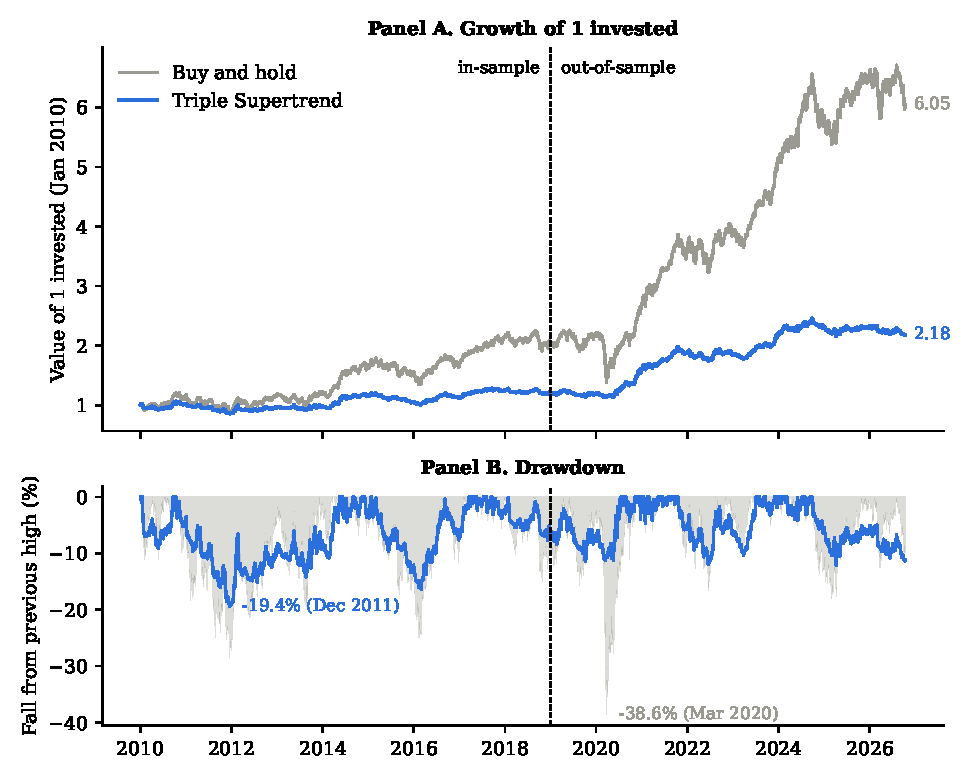
\includegraphics[width=\textwidth]{figures/fig_growth_drawdown.pdf}
\caption{Growth of 1 invested and drawdown from the previous high, equal-weighted point-in-time Nifty~50
members, dividends reinvested, 0.1\% cost per trade. The dashed line separates the in-sample (2010--2018) and
out-of-sample (2019--2026) periods.}
\label{fig:growth}
\end{figure}

Table~\ref{tab:tests} tests whether the differences are statistically meaningful. The return shortfall is borderline
significant in sample ($t = -2.00$) and not significant out of sample. The Sharpe-ratio difference is not
significant in either period, so we cannot reject that the two approaches have equal risk-adjusted returns.

\begin{table}[ht]
\centering
\caption{Strategy minus buy-and-hold: significance tests}
\label{tab:tests}
\small
\begin{tabular}{lrrrr}
\toprule
Period & Mean daily excess & Newey--West $t$ & Sharpe difference [95\% CI] & Bootstrap $p$ \\
\midrule
2010--2018 & $-$2.8 bp & $-$2.00 & $-$0.29 [$-$0.65, 0.06] & 0.097 \\
2019--2026 & $-$3.0 bp & $-$1.58 & $+$0.06 [$-$0.52, 0.69] & 0.996 \\
\bottomrule
\end{tabular}
\end{table}

% ------------------------------------------------------------------------------------------------
\section{Survivorship bias}

Back-filling today's Nifty~50 list into the past roughly doubles buy-and-hold's apparent in-sample return, from
8.7\% to 18.6\% a year (Figure~\ref{fig:surv}). Today's list consists, by construction, of companies that grew
enough to enter or remain in the index; testing on it rewards whichever approach held them longest, which is
buy-and-hold. A trend rule that steps aside from falling stocks gains relatively more from including the failures.
Backtests of Indian trading rules on today's constituents therefore overstate buy-and-hold by 7--10 percentage
points a year and understate the relative case for a trend filter.

\begin{figure}[ht]
\centering
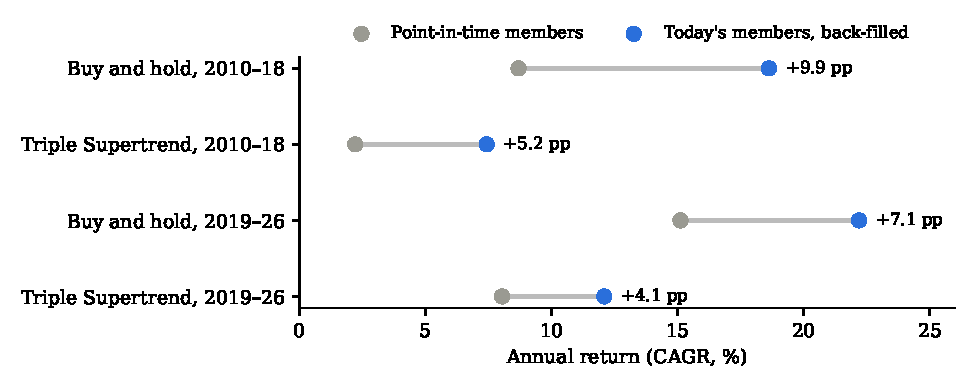
\includegraphics[width=\textwidth]{figures/fig_survivorship.pdf}
\caption{Annual return using point-in-time members versus today's members back-filled into the past.}
\label{fig:surv}
\end{figure}

% ------------------------------------------------------------------------------------------------
\section{Would picking recent winners do better?}

A natural alternative to timing all stocks is to hold only the strongest ones. Choosing the stocks that turned out
best ex post would beat almost any benchmark but is not implementable, so we test cross-sectional momentum, a rule
that uses only past prices. At each month-end $t$, members of the index on $t$ are ranked by
$P_{t}/P_{t-12\,\mathrm{m}} - 1$; the top 10 are held equally weighted from $t+2$ (the signal uses the close of
$t$ and trades at the next close) until the next rebalance. A selected stock is held until the next rebalance even
if it leaves the index; delisted stocks drop out and the rest are re-weighted. Rebalancing costs 0.1\% per side on
turnover, which averages 49\% of the portfolio a month. Twelve variants (top 5, 10 or 15 stocks; 6- or 12-month
lookback; with or without skipping the latest month) were ranked by 2010--2018 Sharpe ratio, and the best was run
unchanged on 2019--2026.

\begin{table}[ht]
\centering
\caption{Momentum (top 10, 12-month lookback) versus buy-and-hold and the Triple Supertrend}
\label{tab:mom}
\small
\begin{tabular}{llrrrr}
\toprule
Period & Portfolio & CAGR & Volatility & Sharpe & Max drawdown \\
\midrule
2019--2026 (out of sample) & Momentum, top 10 & 9.3\% & 20.3\% & 0.54 & $-$36.9\% \\
 & Buy and hold, all members & 15.1\% & 17.4\% & 0.90 & $-$38.6\% \\
 & Triple Supertrend & 8.0\% & 8.5\% & 0.96 & $-$12.1\% \\
Feb 2010--2018 (in sample) & Momentum, top 10 & 13.9\% & 17.3\% & 0.84 & $-$20.4\% \\
 & Buy and hold, all members & 9.4\% & 16.5\% & 0.63 & $-$28.5\% \\
 & Triple Supertrend & 2.8\% & 8.3\% & 0.37 & $-$19.4\% \\
\bottomrule
\end{tabular}

\smallskip
\parbox{0.92\textwidth}{\footnotesize In-sample figures start in February 2010, when momentum first has a full year
of history, and therefore differ slightly from Table~\ref{tab:perf}.}
\end{table}

Momentum beat buy-and-hold in sample but fell well behind out of sample (Table~\ref{tab:mom},
Figure~\ref{fig:mom}). Neither difference is statistically significant: the in-sample Sharpe difference is $+0.22$
(95\% CI $[-0.21, 0.62]$, bootstrap $p = 0.31$) and the out-of-sample difference is $-0.36$ ($[-0.79, 0.05]$,
$p = 0.09$). The out-of-sample shortfall is concentrated in turning points: entering 2020 the rule held the
pre-COVID leaders and gained 1\% that year against 22\% for buy-and-hold, and in January 2023 its holdings
included Adani Enterprises. Within the Nifty~50, momentum gave no reliable edge and was the most volatile of the
three approaches.

\begin{figure}[ht]
\centering
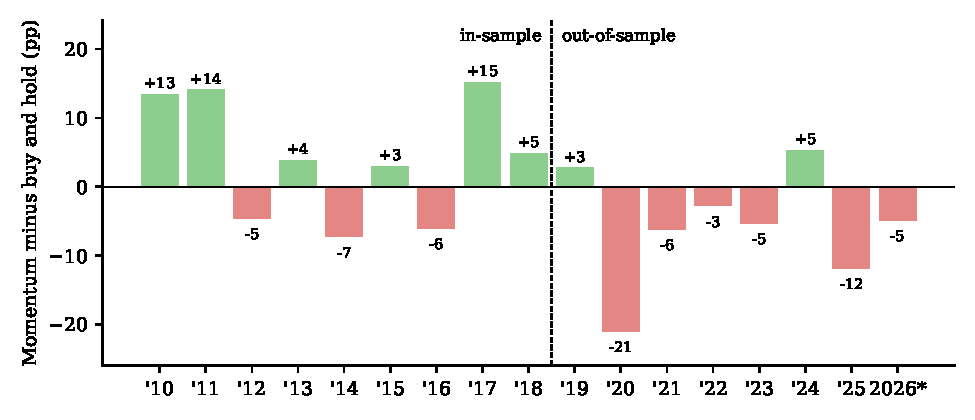
\includegraphics[width=\textwidth]{figures/fig_momentum_by_year.pdf}
\caption{Calendar-year return of top-10 momentum minus equal-weighted buy-and-hold of point-in-time Nifty~50
members, percentage points. *2026 to 9 October.}
\label{fig:mom}
\end{figure}

% ------------------------------------------------------------------------------------------------
\section{Robustness and extensions}

\paragraph{Data source.} Table~\ref{tab:source} repeats the test with three price sets. Each gives roughly half
the return with a similar Sharpe ratio. With Yahoo prices, which lack seven delisted or merged members (4.7\% of
member-days), the in-sample choice moves from exit $(12,3)$ to $(11,2)$, so the parameter choice is sensitive to
data quality.

\begin{table}[ht]
\centering
\caption{Out-of-sample results (2019--2026) by price source}
\label{tab:source}
\small
\begin{tabular}{lcrrrr}
\toprule
Prices & Chosen exit & Strategy CAGR & B\&H CAGR & Strategy Sharpe & B\&H Sharpe \\
\midrule
NSE, total return (main) & (12, 3) & 8.0\% & 15.1\% & 0.96 & 0.90 \\
NSE, price only & (12, 3) & 6.7\% & 13.1\% & 0.81 & 0.79 \\
Yahoo, adjusted & (11, 2) & 6.1\% & 14.8\% & 0.88 & 0.88 \\
\bottomrule
\end{tabular}
\end{table}

\paragraph{Exploratory variants.} Before the formal design, we compared common variants informally on 2018--2026
daily data for two indices, four Nifty stocks and two cryptocurrencies, with no holdout period. A patient
$(12,3)$ exit raised returns on seven of eight assets; a 200-day filter lowered returns on all eight while reducing
drawdowns on seven; weekly bars were worse on six of eight; a MACD$(12,26,9)$ crossover was mixed and traded two to
three times as often; requiring MACD confirmation changed almost nothing; and adding short positions when all three
Supertrends turned down hurt most assets. The rule beat buy-and-hold only on Ethereum and, narrowly, Bitcoin.

\paragraph{Index options.} Buying at-the-money calls on all-green signals and puts on all-red signals lost money
on every index over ten years (Figure~\ref{fig:options}), with options priced by Black--Scholes from India VIX,
one lot per trade and 1\% slippage per side. Most contracts expired before the slow exit fired, so each roll paid
time value again. Only Nifty calls with at least 45 days to expiry broke even, with a peak-to-trough loss of
\rupee3.9 lakh along the way.

\begin{figure}[ht]
\centering
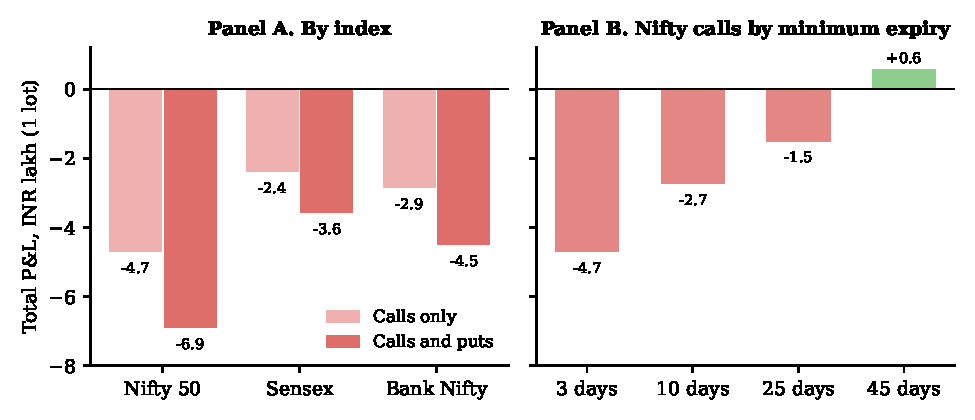
\includegraphics[width=\textwidth]{figures/fig_options.pdf}
\caption{Simulated total profit or loss from buying index options on Triple Supertrend signals over ten years,
INR lakh per lot. Model prices, not traded prices.}
\label{fig:options}
\end{figure}

% ------------------------------------------------------------------------------------------------
\section{Limitations}

The two largest open items both favour the strategy, so the results are, if anything, conservative for it.
Cash earns zero while the strategy is out of the market, whereas Indian Treasury bills paid roughly 4--7\% a year;
this likely understates the strategy by 2--3 percentage points a year. Nor do we yet compare against a static
equity--cash blend of equal volatility, which is the natural benchmark for a rule invested about half the time.
Other limitations are a price-only index benchmark, a flat cost model that ignores rebalancing costs, the
restriction to the Nifty~50, the missing IDFC Ltd series, rights adjustments that omit face value, 120
percentage-of-face-value dividend records that were skipped, and model rather than traded option prices.

Membership files for the Nifty~100, 200 and 500 from the same source were inconsistent: stocks recorded as removed
remained listed in 30 of 46, 42 of 54 and 55 of 75 records respectively, and replaying their change records does
not reconcile. Results on those indices are therefore not reported.

% ------------------------------------------------------------------------------------------------
\section{Conclusion}

On survivorship-free, fully adjusted Nifty~50 data, the Triple Supertrend does not beat buy-and-hold. It earns
about half the return for about half the risk, and its Sharpe ratio is statistically indistinguishable from
buy-and-hold's in both the selection and holdout periods. What the rule reliably delivers is drawdown control:
out of sample its worst drawdown is $-12\%$ against $-39\%$. Concentrating in recent winners does not help
either: top-10 momentum trails buy-and-hold out of sample with the highest volatility of the three approaches.
Whether the Supertrend improves on simply holding less equity is the main open question. Two findings matter beyond this rule: backtests on today's Indian index constituents
overstate buy-and-hold by 7--10 percentage points a year, and NSE's public files can produce a research-quality
panel that includes delisted companies.

\section*{Data and code availability}
All results can be regenerated with the project's scripts: \texttt{fetch\_bhavcopy.py} and
\texttt{fetch\_corp\_actions.py} download NSE data, \texttt{build\_nse\_series.py} links renames and applies
corporate actions and dividends, and \texttt{run\_pit.py -{}-index nifty50 -{}-source nse\_tr} runs the point-in-time
test. Figures are produced by \texttt{paper/make\_figures.py}.

\bibliographystyle{apalike}
\bibliography{references}

\end{document}
